\documentclass{beamer}
\usepackage{progressbar, tcolorbox, CJKutf8, hyperref, multicol, pdfpages, graphicx, xcolor, blindtext, tikz, smartdiagram, listings}
\usepackage[absolute,overlay]{textpos}
\usepackage[backend=bibtex,style=numeric,sorting=none]{biblatex}

\hypersetup{
    colorlinks=true,
    linkcolor=blue,
    filecolor=magenta,      
    urlcolor=blue,
    }

    \definecolor{mygreen}{rgb}{0,0.6,0}
    \definecolor{mygray}{rgb}{0.5,0.5,0.5}
    \definecolor{mymauve}{rgb}{0.58,0,0.82}


    \lstset{ 
      backgroundcolor=\color{white},   % choose the background color; you must add \usepackage{color} or \usepackage{xcolor}; should come as last argument
      basicstyle=\ttfamily\footnotesize,% the size of the fonts that are used for the code
      breakatwhitespace=false,         % sets if automatic breaks should only happen at whitespace
      breaklines=true,                 % sets automatic line breaking
      captionpos=b,                    % sets the caption-position to bottom
      commentstyle=\color{mygreen},    % comment style
      deletekeywords={...},            % if you want to delete keywords from the given language
      escapeinside={\%*}{*)},          % if you want to add LaTeX within your code
      extendedchars=true,              % lets you use non-ASCII characters; for 8-bits encodings only, does not work with UTF-8
      frame=single,	                   % adds a frame around the code
      keepspaces=true,                 % keeps spaces in text, useful for keeping indentation of code (possibly needs columns=flexible)
      keywordstyle=\color{magenta},        % keyword style
      morekeywords={FROM, RUN, ENV, USER, WORKDIR, CMD, EXPOSE, ADD, COPY, sudo, curl, chmod, ln, git, cd},
                                       % if you want to add more keywords to the set
      numbers=left,                    % where to put the line-numbers; possible values are (none, left, right)
      numbersep=5pt,                   % how far the line-numbers are from the code
      numberstyle=\tiny\color{mygray}, % the style that is used for the line-numbers
      rulecolor=\color{black},         % if not set, the frame-color may be changed on line-breaks within not-black text (e.g. comments (green here))
      showspaces=false,                % show spaces everywhere adding particular underscores; it overrides 'showstringspaces'
      showstringspaces=false,          % underline spaces within strings only
      showtabs=false,                  % show tabs within strings adding particular underscores
      stepnumber=1,                    % the step between two line-numbers. If it's 1, each line will be numbered
      stringstyle=\color{mymauve},     % string literal style
      tabsize=4,	                     % sets default tabsize to ˋ spaces
      title=\lstname
    }

\graphicspath{ {./images/} }
\usetheme{AnnArbor}
\addbibresource{main.bib}
\usetikzlibrary{positioning, calc, shapes.multipart, shapes.arrows, fit, backgrounds}

\definecolor{dockerColor}{RGB}{13, 183, 237}
\definecolor{secureColor}{RGB}{10, 191, 83}
\definecolor{aquamarine}{rgb}{0.5, 1.0, 0.83}
\definecolor{aquamarine2}{rgb}{0.2, 1.0, 0.53}

\title{The Container Security in Healthcare Data Exchange System}
\subtitle{Bachelor's degree graduation project}
\author{Chih-Hsuan Yang}
\institute{National Sun Yat-sen University\\
Advisor: Chun-I Fan
}
\date{\today}

\AtBeginSection[]{
  \begin{frame}
  \vfill
  \centering
  \begin{beamercolorbox}[sep=8pt,center,shadow=true,rounded=true]{title}
    \usebeamerfont{title}\insertsectionhead\par%
  \end{beamercolorbox}
  \vfill
  \end{frame}
}

\def\checkmark{\tikz\fill[scale=0.4](0,.35) -- (.25,0) -- (1,.7) -- (.25,.15) -- cycle;} 

\begin{document}
\begin{CJK*}{UTF8}{bsmi}

  \begin{frame}
    \titlepage
  \end{frame}


  \begin{frame}{Outline}
    \begin{multicols}{2}
      \tableofcontents
    \end{multicols}
  \end{frame}

  \begin{frame}{Flow chart}
    \centering
    \scalebox{0.9} {
      \smartdiagram[flow diagram:horizontal]{
        Scan base, Sign, Image checking, Start policy, Runtime enforcement
      }
    }
  \end{frame}


  \begin{frame}{Plans in this week}
    \begin{itemize}
      \item Use the BPF feature and fuzzing technique to collect the "normal" system calls in healthcare data exchange system.
      \item Keep survey those papers.
    \end{itemize}
  \end{frame}

  \section{Last week}
  \begin{frame}
    \begin{itemize}
      \item (e)BPF is a dynamic tracing technique.
      \item The bpf() system call first appeared in Linux 3.18.
      \item The kernel provide a JIT that can execute out Byte Code probe into the kernel dynamically.
    \end{itemize}
  \end{frame}

  \begin{frame}{cannot attach kprobe, probe entry may not exist}
    \begin{multicols*}{2}
      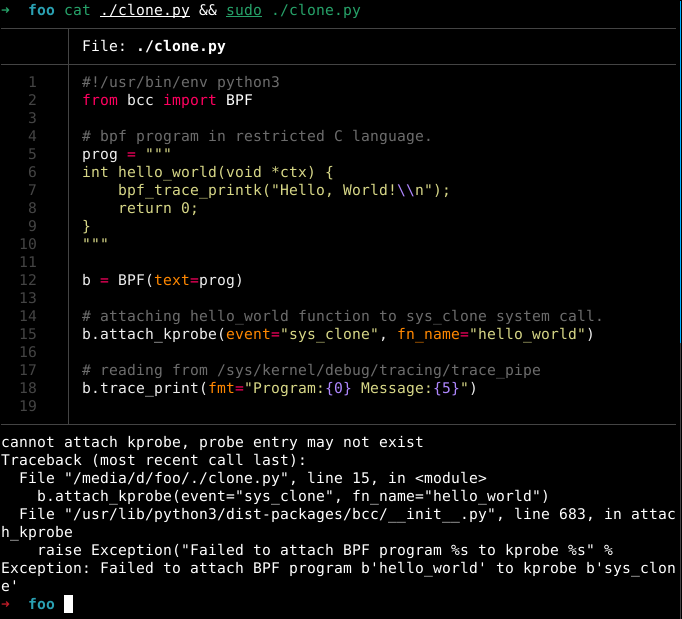
\includegraphics[width=.7\textwidth]{Qbrd44D.png}
      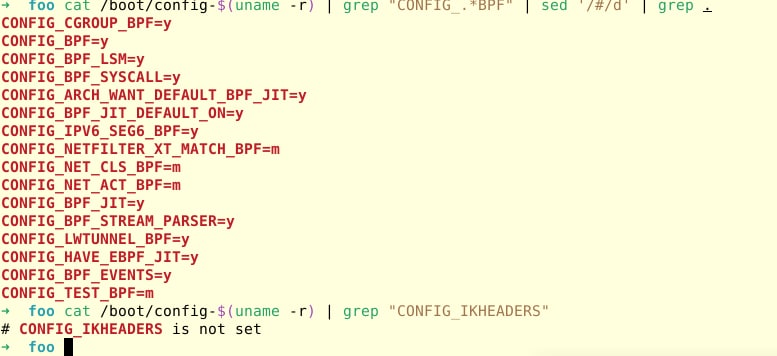
\includegraphics[width=.5\textwidth]{yEC8xkQ.png}
    \end{multicols*}
  \end{frame}


  \begin{frame}{Recompile the kernel}
    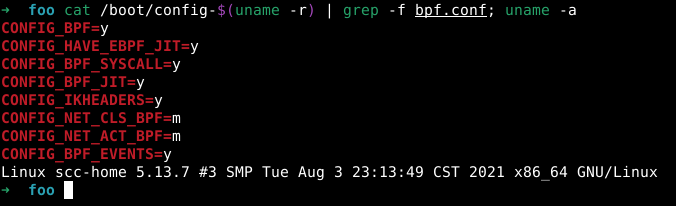
\includegraphics[width=\textwidth]{7OTOHXg.png}\\
    But it still not work, which has same error as previous.
  \end{frame}

  \begin{frame}{Another front-end wrapper bpftrace}
    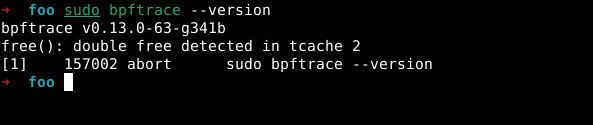
\includegraphics[width=\textwidth]{eU4xGbt.png}\\
    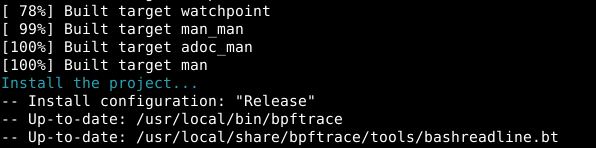
\includegraphics[width=\textwidth]{SHtVxmB.png}\\
    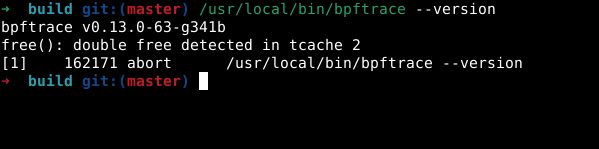
\includegraphics[width=\textwidth]{W4JhZcO.png}
  \end{frame}

  \begin{frame}{bpftrace using docker}
    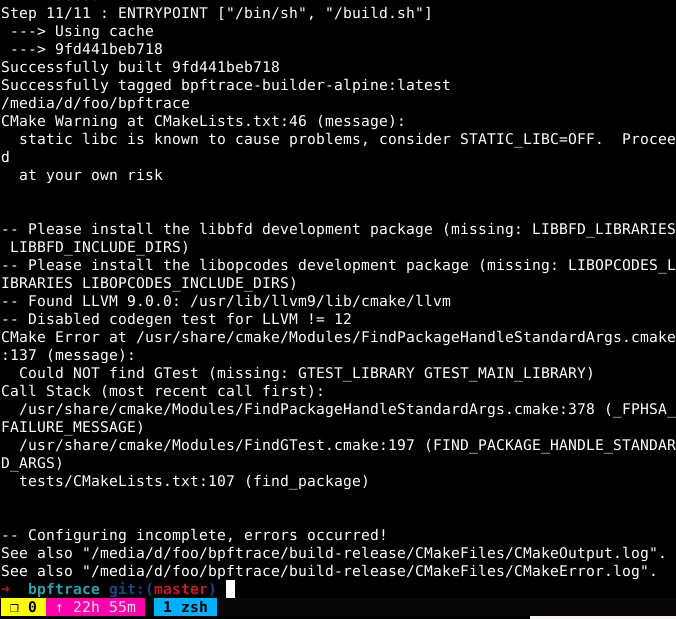
\includegraphics[height=.8\textheight]{f6GBfST.png}
    \url{https://hackmd.io/@25077667/Byvwszd1K\#bpftrace-using-docker}
  \end{frame}

  \begin{frame}{The official document says}
    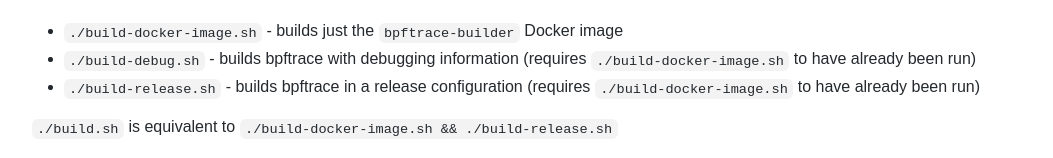
\includegraphics[width=\textwidth]{Screenshot_2021-08-06_06-50-18.png}
    \begin{multicols*}{2}
      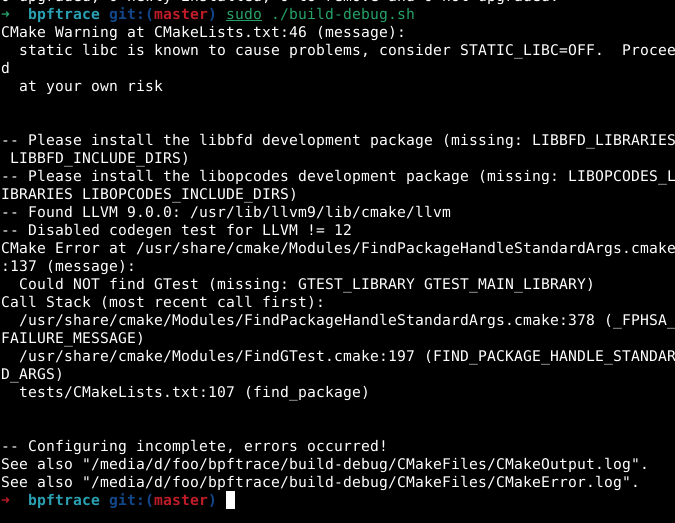
\includegraphics[height=.6\textheight]{C86IdNH.png}
      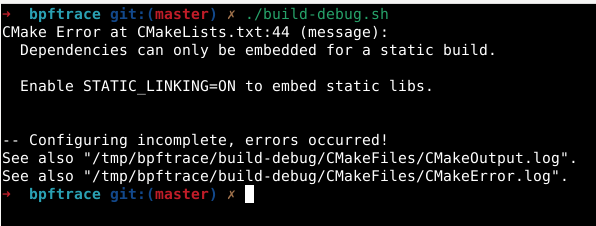
\includegraphics[height=.6\textheight]{Screenshot_2021-08-06_07-00-24.png}
    \end{multicols*}

  \end{frame}

  \begin{frame}
    \centering
    
\includegraphics[height=\textheight]{photo_2021-08-04_02-25-37.jpg}
  \end{frame}

  \begin{frame}{Debends on kernel version and distro.}
    \begin{multicols*}{2}
      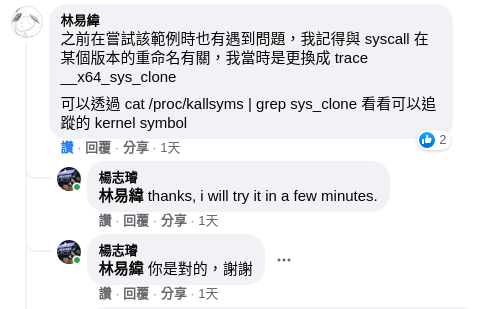
\includegraphics[width=.5\textwidth]{Screenshot_2021-08-06_06-22-21.png}
      
\includegraphics[width=.5\textwidth]{Screenshot_2021-08-06_06-22-40.png}
    \end{multicols*}
  \end{frame}

  \begin{frame}{Many debugs\dots}
    \begin{itemize}
      \item The kernel what I compiled is 5.13.7.
      \item Hey, there are no `linux-headers-\$(uname -a)` in debian sid!
      \item Okay, I can compile the header my my self.
      \item Hey, the bcc and bpftrace are failed, they cannot get those entry on 5.13.7.
      \item Okay, I go to fix the bcc and bpftrace source code, and it works on host OS.
      \item Hey, It does not work in container, failed to compile BPF module. (Next page)
      \item Okay, I change the front end of eBPF to tracee, which is another open source wrapper.
      \item It also works on host OS, but failed to load libbpf in container. (Next page)
    \end{itemize}
  \end{frame}

  \begin{frame}
    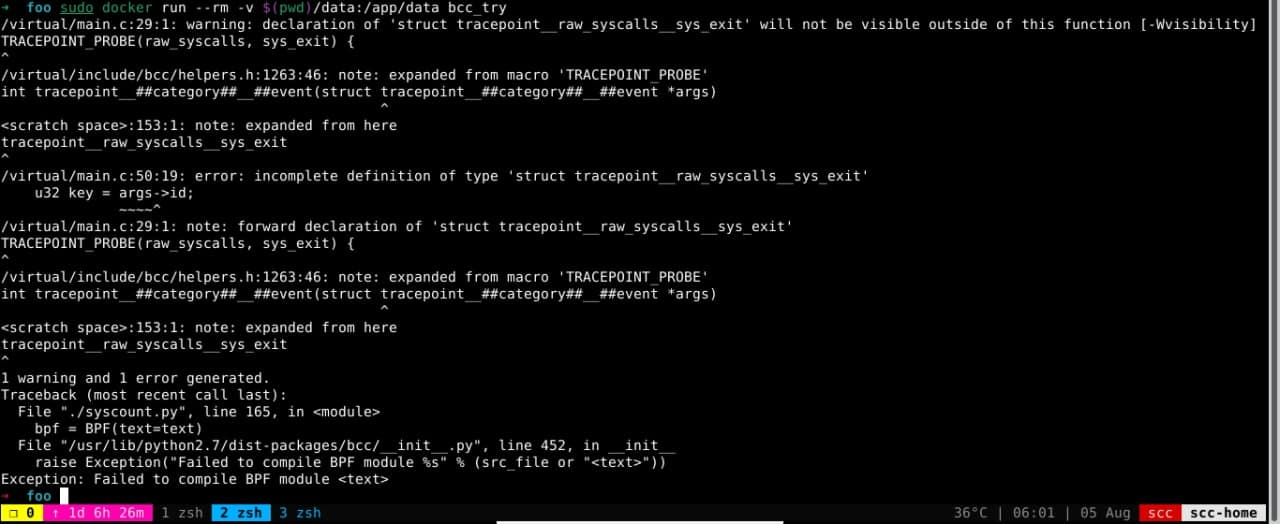
\includegraphics[height=.5\textheight]{photo_2021-08-05_06-02-50.jpg}
    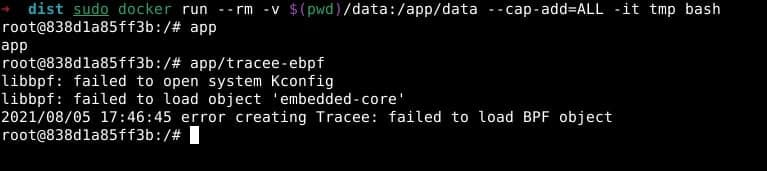
\includegraphics[height=.5\textheight]{photo_2021-08-06_02-08-38.jpg}
  \end{frame}

  \begin{frame}{There also have some distro. dependency issue}
    \begin{itemize}
      \item Alpine
      \item Debian stretch, buster, bulleyes
      \item Ubuntu Bionic, Focal Fossa
      \item Linux kernel version, 4.18.0, 5.2.0\dots
    \end{itemize}
    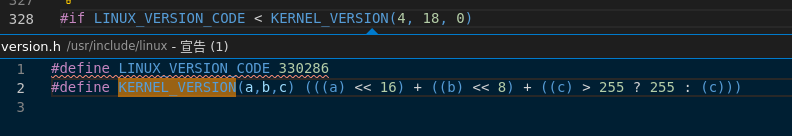
\includegraphics[width=\textwidth]{Screenshot_2021-08-06_06-44-54.png}
    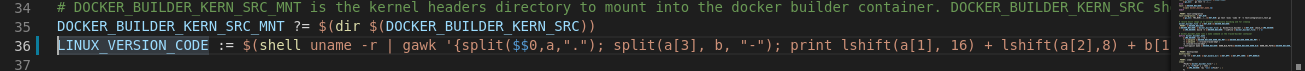
\includegraphics[width=\textwidth]{Screenshot_2021-08-06_06-46-24.png}
  \end{frame}

  \section{This week}
  \begin{frame}{Can work on "Simple" test case}
    \lstinputlisting{src/hello.py}
    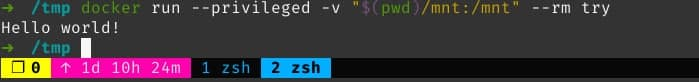
\includegraphics[width=\textwidth]{photo_2021-08-13_12-20-31.jpg}
  \end{frame}

  \begin{frame}
    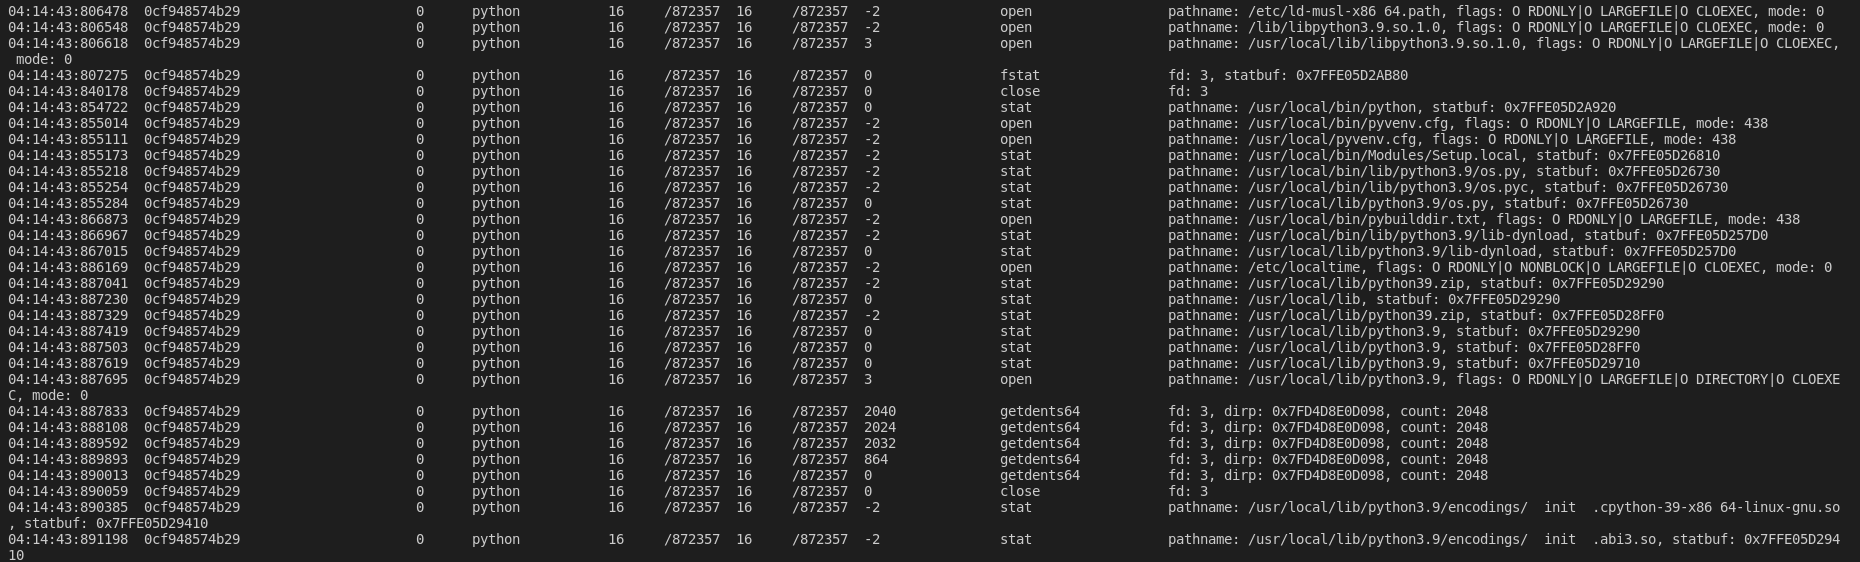
\includegraphics[width=\textwidth]{Screenshot_2021-08-13_12-30-53.png}
    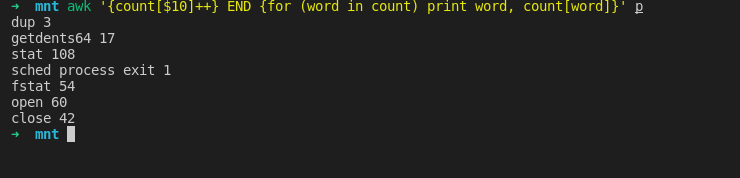
\includegraphics[width=\textwidth]{Screenshot_2021-08-13_12-29-19.png}
    We didn't catch the `write' system call, that is if there is a process called `write'.\\
    It's invalid operation.
    Even though it is a common system call.
  \end{frame}

  \begin{frame}{Move the ebpf bin to the FHIR Env.}
    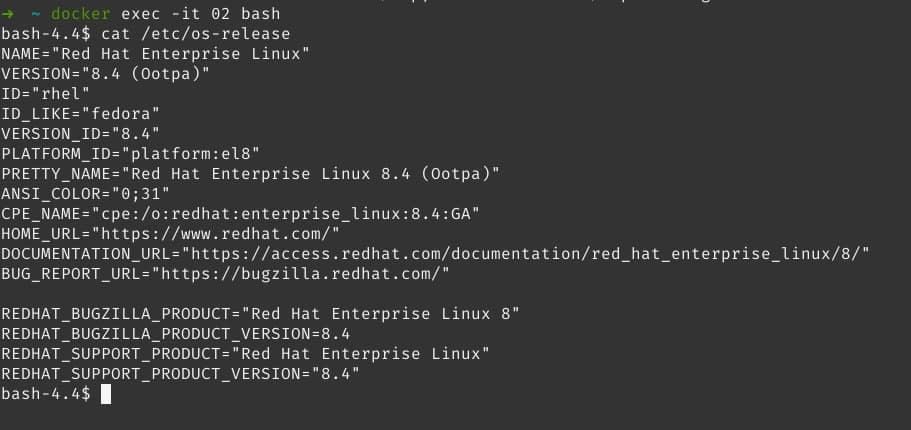
\includegraphics[width=\textwidth]{photo_2021-08-13_07-03-33.jpg}
  \end{frame}

  \begin{frame}
    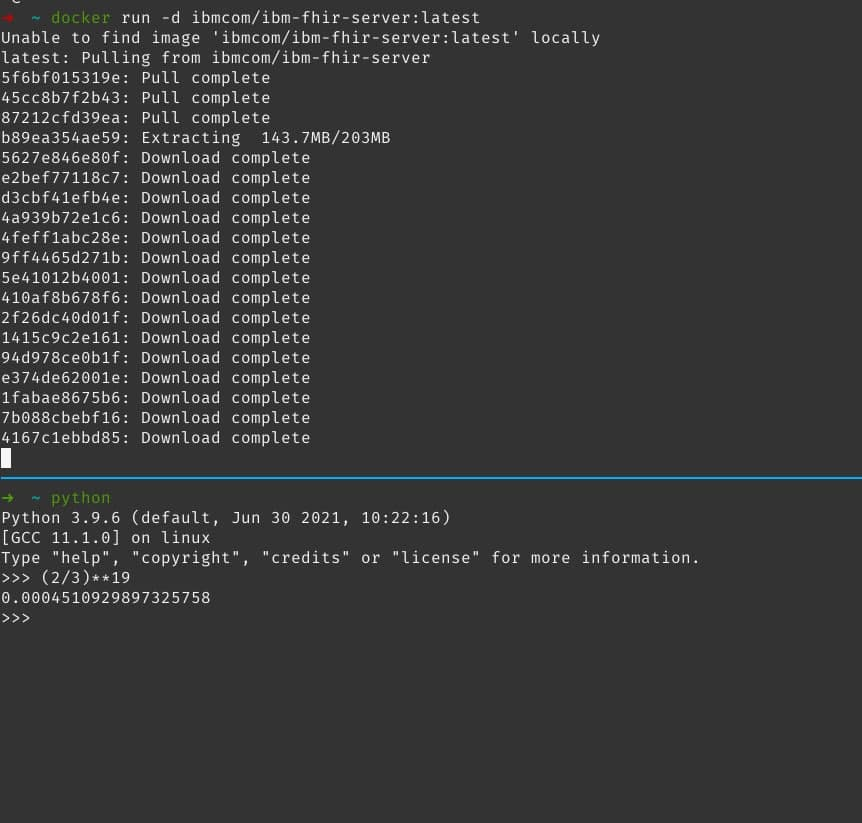
\includegraphics[width=\textwidth]{photo_2021-08-13_07-00-50.jpg}
  \end{frame}

  \begin{frame}
    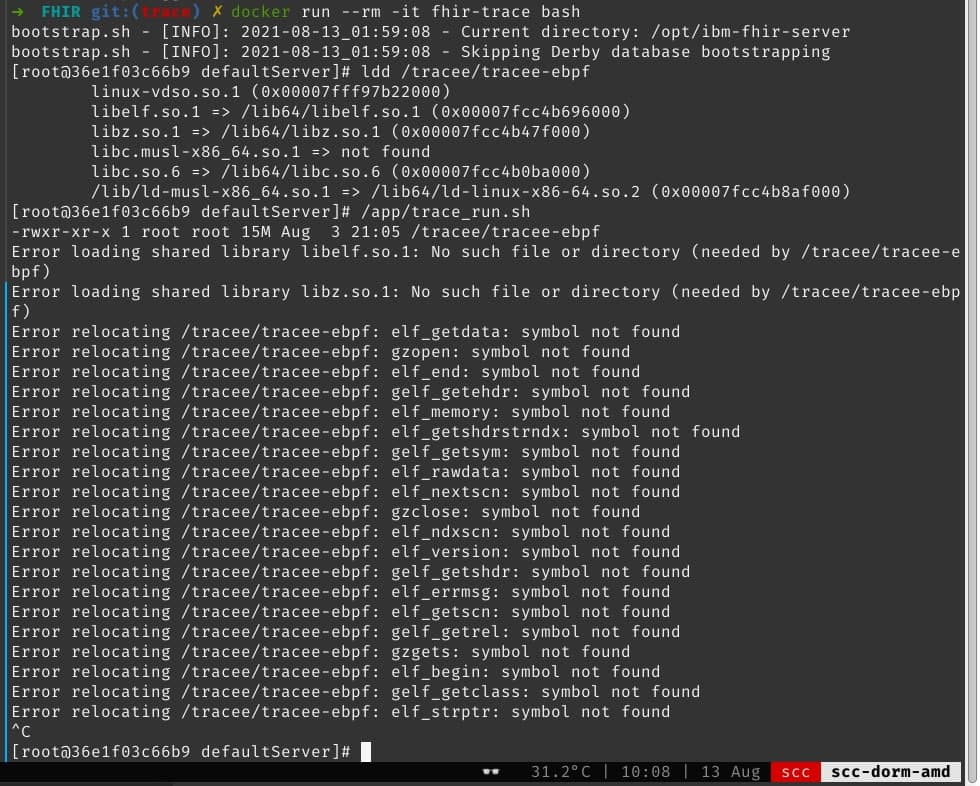
\includegraphics[width=\textwidth]{photo_2021-08-13_10-12-53.jpg}
  \end{frame}

  \begin{frame}{Lisense issue? self-build!}
    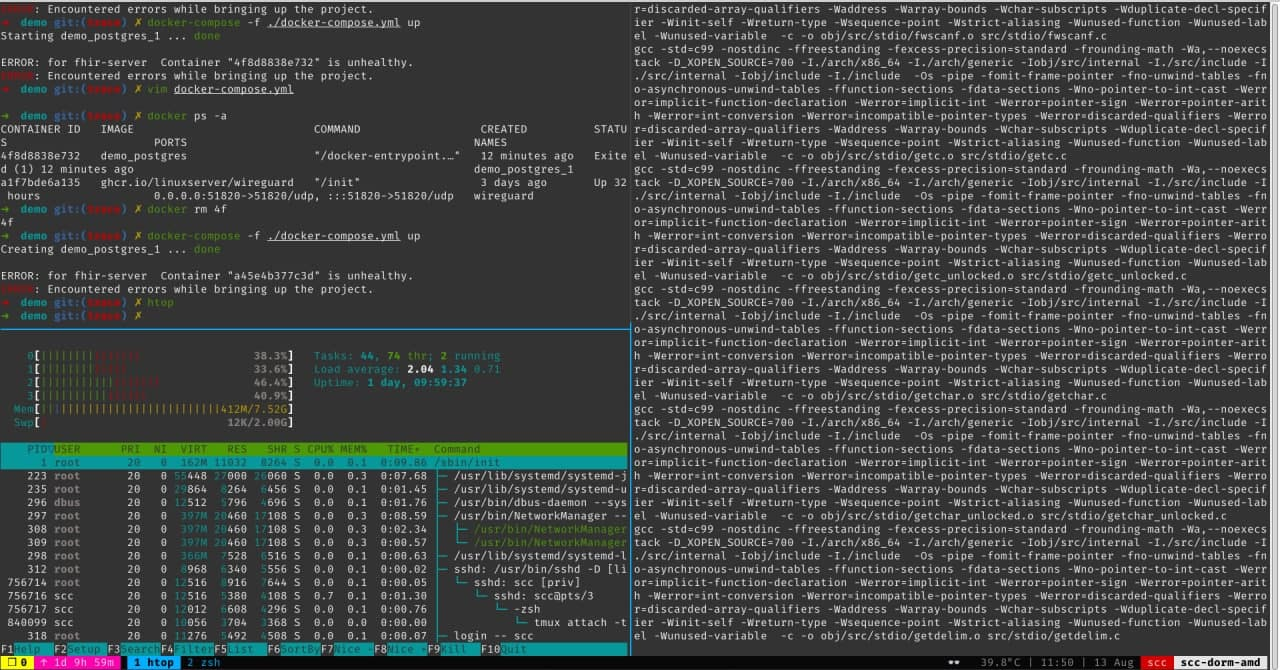
\includegraphics[width=\textwidth]{photo_2021-08-13_11-55-21.jpg}
  \end{frame}

  \begin{frame}{Well\dots}
    \begin{multicols*}{2}
      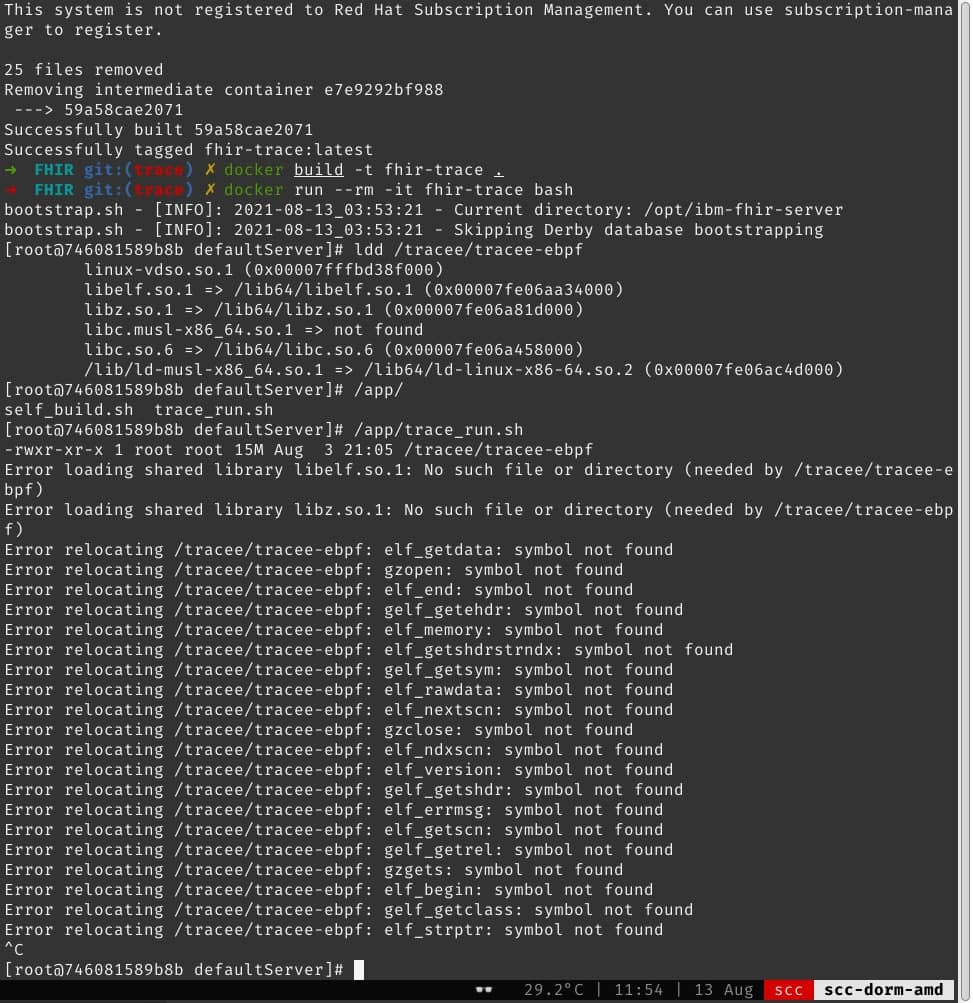
\includegraphics[width=.5\textwidth]{photo_2021-08-13_12-55-41.jpg}
      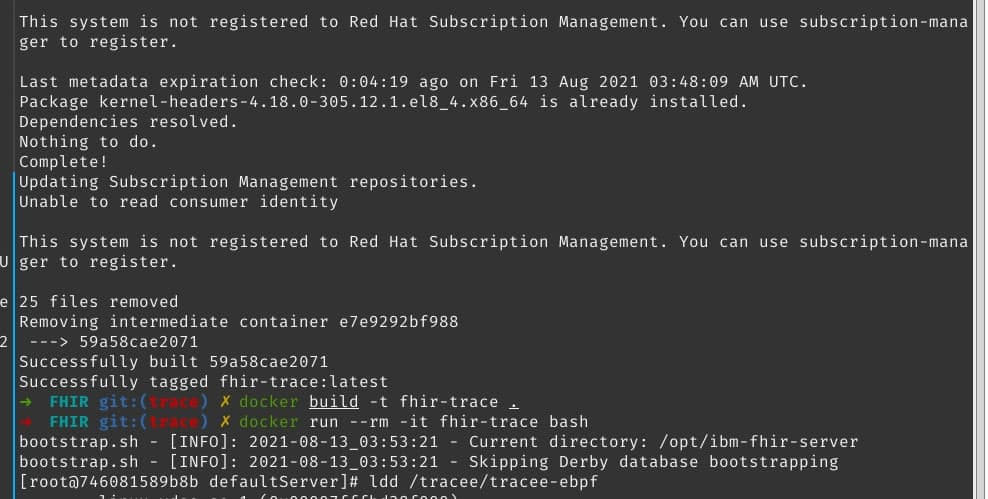
\includegraphics[width=.5\textwidth]{photo_2021-08-13_12-02-09.jpg}
    \end{multicols*}
  \end{frame}

  \begin{frame}
    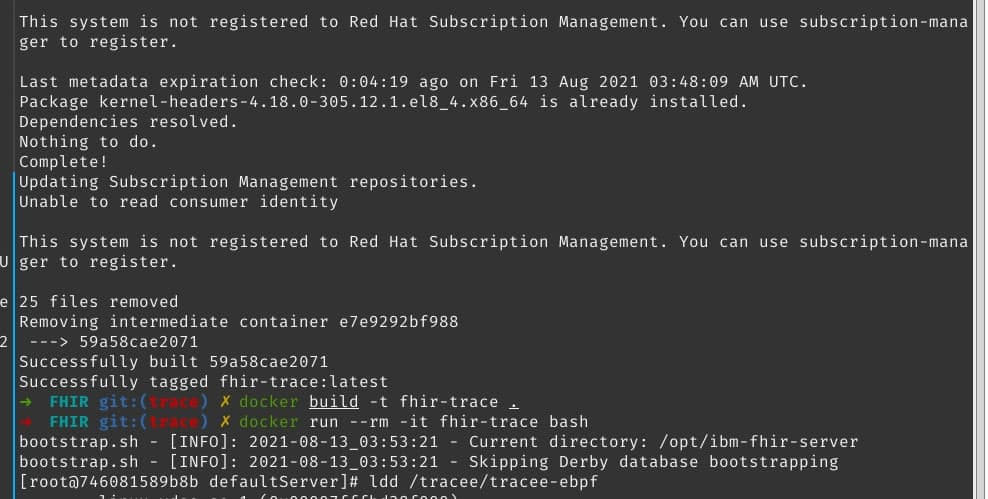
\includegraphics[width=\textwidth]{photo_2021-08-13_12-02-09.jpg}
  \end{frame}

  \begin{frame}{3 problems to be solve}
    \begin{enumerate}
      \item Kernel version
      \item Dynamic linking issue: musl, libelf
      \item Has it enough time to fuzz?
    \end{enumerate}
  \end{frame}

\end{CJK*}
\end{document}